\documentclass[conference]{IEEEtran}

\usepackage[english]{babel} 
\usepackage[utf8]{inputenc}
\usepackage[T1]{fontenc}
\usepackage{cite}
\usepackage{url}
\usepackage{hyphenat} % For linebreaks
\usepackage{hyperref}
\usepackage{geometry}
\usepackage{graphicx} % IncludeGraphis
\usepackage{caption} % Subfigure
\usepackage{subcaption} % Subfigure
\usepackage{lipsum} % Lorem Ipsum dummy text

% correct bad hyphenation here
% \hyphenation{op-tical net-works semi-conduc-tor}


\begin{document}

\title{Stream processing with Twitter Heron}

\author{\IEEEauthorblockN{Adrian Bartnik}
\IEEEauthorblockA{Technische Universität Berlin\\
Email: bartnik@campus.tu-berlin.de}}

\maketitle

\begin{abstract}
This paper gives an overview about the requirements and the demands of a real-time stream processing platform.
As an example, it presents the architecture and design decisions of Apache Storm, its successor Twitter Heron and Google`s MillWheel. % Asumptions?
It compares each streaming platform in terms of prior assumptions, scalability and extensibility.
Finally, it presents a summary with the advantages and disadvantages of each platform and gives an outlook for future use cases.

\end{abstract}

\section{Introduction}
\label{sec:Introduction}

In recent years, stream processing has become a new companion to the family of big data buzzwords.
It describes the paradigm of processing incoming high-volume data stream, where the data can come from various sources.
Scenarios are micro transactions at a stock exchange, sensor measurements from small independent devices in the upcoming area of the Internet of Things or analytic data coming in from millions of mobile phones.

Most major Internet-scale companies either have their own proprietary stream processing platform or use some open-source alternative.
One prominent example is Twitter, a real-time messaging service with over 320 million active users and over 1 billion unique site visits each month.
Twitter uses stream processing in various places, for example to compute the trending topics, a small section on their website showing the currently most used, and therefore most relevant keywords by their users.
In 2011 Twitter started off developing its own stream processing platform Twitter Storm after acquiring the technology from the company BackType.
Shortly afterwards, they also made the whole project available under open source and it became an Apache top-level project.

But, using Storm at its scale was becoming increasingly challenging due to issues related to scalability, debug-ability, manageability, and efficient sharing of cluster resources with other data services.
The company therefore started to develop a new system, Twitter Heron, which should fix their problems and also be able to scale for the future.
Twitter Heron is now the de facto stream data processing platform inside Twitter.

The rest of the paper is organized as follows: The following section, Section \ref{sec:Background}, describes the characteristics of real-time stream processing and the requirements of a stream processing platform.
Section \ref{sec:RelatedWork} describes other platforms and related work.
Section \ref{sec:ApacheStorm} and \ref{sec:TwitterHeron} describe Apache Strom and Titter Heron respectively, where the later also describes the evolution between the two platform.
The evaluation in section \ref{sec:Evaluation} compares both approaches.
Finally, section \ref{sec:Conclusion} contains the conclusion.

\section{Background}
\label{sec:Background}

This section explains the fundamentals of stream processing and the characteristics and requirements of a stream processing platform respectively.

\subsection{Real-time Stream Processing}
\label{sec:RealTimeStreamProcessing}

The major distinction between plain big data and stream processing is, that the later operates on \emph{unbounded data}.
This means, that the size of the input is ever-growing and essentially infinite, whereas usually the input size is typically limited by either the file or database size and known in advance \cite{WorldBeyondBatch}.

Generally speaking, stream processing describes a one-at-a-time processing model, where each data item is arriving separately and is independent from the rest.
This holds true for most use cases, such as financial transactions, sensor measurements from different devices or in Twitter's case \emph{tweets}.
As results should be available as fast as possible, the items should be process upon arrival and not be combined into batches.
The goal is typically to achieve sub-second latency \cite{BeyondBatchProcessing}.

The computations of a stream processing platform on the incoming data should ideally be simple, independent and separated.
This way it becomes easier to distribute the computations onto different machines in one cluster and thus the whole platform can scale better.
In many systems the computations on the data form a directed acyclic graph, e.g. the jobgraph in Flink or, as we will see, a topology in Heron \cite{Flink}.
Finally, all computations should happen in-memory, because writing intermediate results to disk would introduce a big delay compared to pure memory access.

\subsection{Requirements of a Stream Processing Platform}
\label{sec:RequirementsOfAStreamProcessingPlatform}

In 2005, Michael Stonebraker et al. outlined eight requirements that a system should meet to excel at a variety of real-time stream processing applications.
They provide high-level guidance when evaluating alternative solutions \cite{The8Requirements}.
Later on, these requirements will be compared to Apache Storm and Twitter Heron.

\begin{LaTeXdescription}
  \item[1) Keep the data moving] The data should be processed \emph{in-stream}, without a requirement to be stored on disk to perform additional operations
  \item[2) Query using SQL on Streams] Support a high-level “StreamSQL” language with built-in extensible stream-oriented primitives and operators.
  \item[3) Handle Stream Imperfections] Provide resiliency against stream “imperfections”, including delayed, missing and out-of-order data.
  \item[4) Generate Predictable Outcomes] A stream processing platform must guarantee predictable and repeatable outcomes.
  \item[5) Integrate Stored and Streaming Data] The system should be able to integrate live and stored data seamlessly and to have the capability to efficiently store, access and modify state information.
  \item[6) Guarantee Data Safety and Availability] Ensure that the system is up and available, and the integrity of the data maintained at all times, despite failures.
  \item[7) Partition and Scale Applications Automatically] The system should enable incremental scalability across multiple processors or machines, ideally automatically and transparent.
  \item[8) Process and Respond Instantaneously] The stream processing system must have a highly-optimized, minimal-overhead execution engine to deliver real-time response for high-volume applications.
\end{LaTeXdescription}

\begin{figure*}[!h]
\centering
	\begin{subfigure}{.55\columnwidth}
		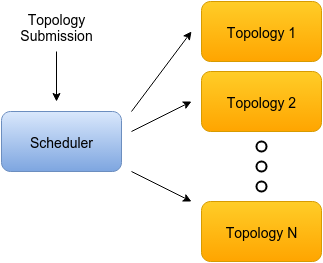
\includegraphics[width=\columnwidth]{figures/TopologySubmission}
		\caption{The overview of the \\topology submission}
		\label{fig:TopologySubmission}
	\end{subfigure}\hspace{2.9em}
	\begin{subfigure}{1.35\columnwidth}
		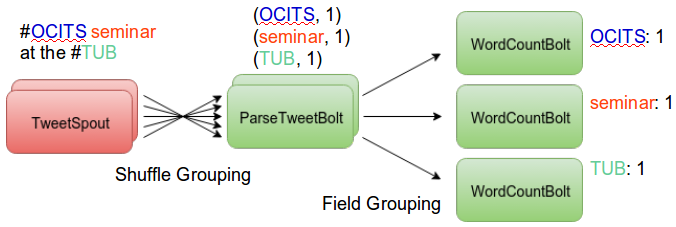
\includegraphics[width=\columnwidth]{figures/TopologyWordCount}
		\caption{An example wordcount topology}
		\label{fig:TopologyWordcount}
	\end{subfigure}\hfill
\label{TopologyDescription}
\caption{Overview of the topologies in Apache Storm and Twitter Heron}
\end{figure*}

\section{Related Work}
\label{sec:RelatedWork}

\lipsum[2-6]


\cite{InfoQGameChanger}



\section{Apache Storm}
\label{sec:ApacheStorm}


\begin{figure*}[!h]
\centering
	\begin{subfigure}{.55\columnwidth}
		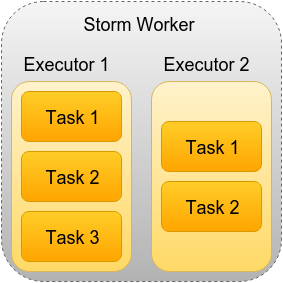
\includegraphics[scale=0.45]{figures/StormWorker}
		    \caption{The overview of the Storm worker}
		    \label{fig:StormWorkerOverview}
	\end{subfigure}\hspace{2.9em}
	\begin{subfigure}{1.35\columnwidth}
		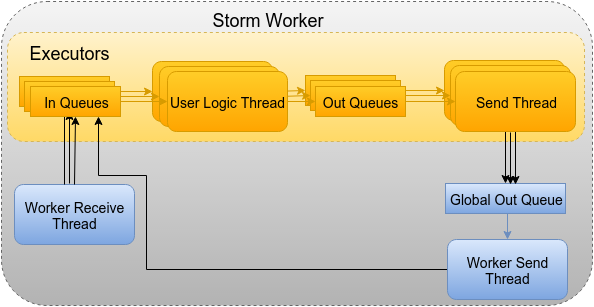
\includegraphics[scale=0.45]{figures/StormWorkerDetail}
		    \caption{The internals of the Storm worker}
		    \label{fig:StormWorkerDetail}
	\end{subfigure}\hfill
\label{StormOverview}
\caption{Overview of Apache Storm architecture}
\end{figure*}


\lipsum[2-3]


\subsection{Data model}

\lipsum[2-4]

\subsection{Architecture}

\lipsum[2-4]

\cite{StormTwitter}

\section{Twitter Heron}
\label{sec:TwitterHeron}

\lipsum[2-4]


\subsection{Evolution from Apache Storm}
\label{sec:EvolutionFromApacheStorm}

\lipsum[2-4]


\subsection{Twitter Heron Architecture}
\label{sec:TwitterHeronArchitecture}

\lipsum[2-4]


\begin{figure*}[!tp]
    \centering
    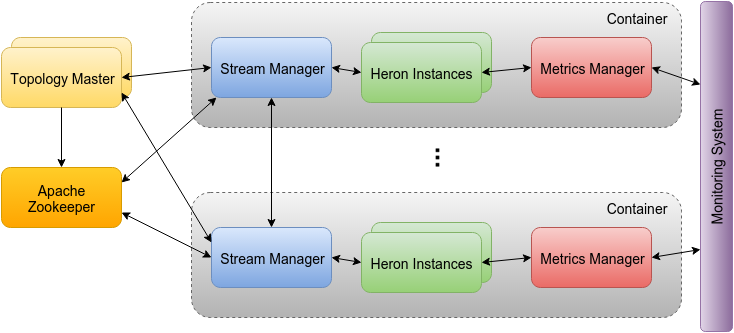
\includegraphics[scale=0.45]{figures/HeronOverview}
    \caption{The overview of Heron}
    \label{fig:HeronOverview}
\end{figure*}

\begin{figure*}[htp]
    \centering
    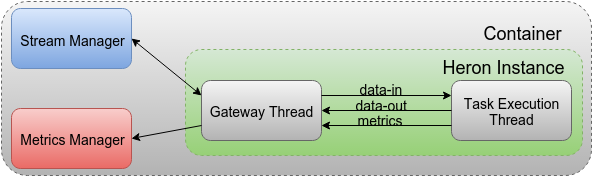
\includegraphics[scale=0.45]{figures/HeronInstance}
    \caption{The internals of a Heron Instance}
    \label{fig:HeronInstance}
\end{figure*}

\cite{ElasticScalingStreamProcessing}
\cite{OnlyOneLook}
\cite{YARN}
\cite{ScalableDistributedStreamProcessing}

% \section{Google MillWheel}

% \cite{Millwheel}

\section{Evaluation}
\label{sec:Evaluation}

\lipsum[2-4]


\cite{TwitterHeronBlog}

\cite{TwitterHeron}

Reference 8 requirements \ref{sec:RequirementsOfAStreamProcessingPlatform}.


\section{Conclusion}
\label{sec:Conclusion}

The conclusion goes here.

\lipsum[2-4]



% References

\bibliographystyle{plain} %Choose a bibliograhpic style
\bibliography{Bibliography}

\end{document}